\documentclass{ntmanuscript}
%\usepackage[acronym,toc]{glossaries}
%\include{acros}
%\makeglossaries
%%%%%%%%%%%%%%%%%%%%%%%%%%%%%%%%%%%
\title{Non-judgemental Dynamic Fuel Cycle Benchmarking}

% Authors. Separated by commas
\author{Anthony Michael Scopatz$^1$}

% Institutes of the authors
\institute{$^1$University of South Carolina, Department of Mechanical
    Engineering, Nuclear Engineering Program, Columbia, SC 29201}

% Information concerning the person submitting the manuscript
\submitter{Anthony M. Scopatz}
\submitteraddress{541 Main Street, Columbia, SC 29208}
\submitteremail{scopatz@cec.sc.edu}


% No more than three keywords, though each can be a phrase
\keywords{nuclear fuel cycle, gaussian process, dynamic time warping}

\usepackage{color}
\usepackage{graphicx}
\usepackage{booktabs} % nice rules for tables
\usepackage{microtype} % if using PDF
\usepackage{xspace}
\usepackage{listings}
\usepackage{textcomp}
\usepackage[normalem]{ulem}
\usepackage{amssymb}
\DeclareMathAlphabet{\mathpzc}{OT1}{pzc}{m}{it}

\definecolor{listinggray}{gray}{0.9}
\definecolor{lbcolor}{rgb}{0.9,0.9,0.9}
\lstset{
    %backgroundcolor=\color{lbcolor},
    language={C++},
    tabsize=4,
    rulecolor=\color{black},
    upquote=true,
    aboveskip={1.5\baselineskip},
    belowskip={1.5\baselineskip},
    columns=fixed,
    extendedchars=true,
    breaklines=true,
    prebreak=\raisebox{0ex}[0ex][0ex]{\ensuremath{\hookleftarrow}},
    frame=single,
    showtabs=false,
    showspaces=false,
    showstringspaces=false,
    basicstyle=\scriptsize\ttfamily\color{green!40!black},
    keywordstyle=\color[rgb]{0,0,1.0},
    commentstyle=\color[rgb]{0.133,0.545,0.133},
    stringstyle=\color[rgb]{0.627,0.126,0.941},
    numberstyle=\color[rgb]{0,1,0},
    identifierstyle=\color{black},
    captionpos=t,
}

\newcommand{\code}[1]{\lstinline[basicstyle=\ttfamily\color{green!40!black}]|#1|}
\newcommand{\units}[1] {\:\text{#1}}%
\newcommand{\SN}{S$_N$}
\newcommand{\cyclus}{\textsc{Cyclus}\xspace}
\newcommand{\Cyclus}{\cyclus}
\newcommand{\citeme}{\textcolor{red}{CITE}\xspace}
\newcommand{\cycpp}{\code{cycpp}\xspace}
\newcommand{\TODO}[1] {{\color{red}\textbf{TODO: #1}}}%

\newcommand{\comment}[1]{{\color{green}\textbf{#1}}}

\newcommand{\E}{\mathbb{E}}
\newcommand{\GP}{\mathpzc{GP}}
\newcommand{\LWR}{\mathrm{LWR}}
\newcommand{\FR}{\mathrm{FR}}
\newcommand{\Total}{\mathrm{Total}}
\newcommand{\argmin}{\mathrm{argmin}}
\newcommand{\CYCLUS}{\mathrm{Cyclus}}
\newcommand{\DYMOND}{\mathrm{DYMOND}}
\newcommand{\I}{\mathbf{I}}
\newcommand{\K}{\mathbf{K}}


\date{}
%%%%%%%%%%%%%%%%%%%%%%%%%%%%%%%%%%%
\begin{document}

\begin{abstract}
This paper presents a new fuel cycle benchmarking analysis methodology
by coupling Gaussian process regression, a popular technique in Machine
Learning, to dynamic time warping, a mechanism widely used in speech
recognition. Together they generate figures-of-merit for a suite of fuel
cycle realizations. The figures-of-merit may be computed for any time
series metric that is of interest to a benchmark. For a given metric,
these figures-of-merit have the advantage that they reduce the
dimensionality to a scalar and are thus directly comparable.
The figures-of-merit
account for uncertainty in the metric itself, utilize information
across the whole time domain, and do not require that the simulators
use a common time grid. Here, a distance measure is defined that can be used
to compare the performance of each simulator for a given metric. Additionally,
a contribution measure is derived from the distance measure that can be used
to rank order the impact of different partitions of a fuel cycle metric.
Lastly, this paper
warns against using standard signal processing techniques for error reduction,
as error reduction is better handled by the Gaussian process regression
itself.
\end{abstract}

\section{Introduction}
\label{intro}
The act of fuel cycle benchmarking has long faced methodological issues 
on what metrics to compare, how to compare them, and at what point in the
fuel cycle they should be compared. This is partly because such activities 
are not benchmarking in the strictess validation sense. Most fuel
cycle benchmarks are more correctly called code-to-code comparisons or 
inter-code comparisons, as they compare simultor results. Importantly, 
these take place in the absence of true experimental data. The number of 
real-world, industrial scale nuclear fuel cycles that have historically been 
deployed is not sufficient for statistical accuracy even for the Once-Through 
sceanario. For other fuel cycles, industrial data is even more stark. 
Since fuel cycle simulation is thus effectively impossible to validate, 
we should look to methods non-judgemental methods of benchmarking. The 
results of any given simulator should be evaluated in reference to how 
it performs against other simulators in such a way that acknowledges that 
any and all simulators may demonstrate incorrect behaviour. No simulator
by fiat produces the `true' or reference case.

The other major conceptual issue with fuel cycle benchmarking is that there 
is no agreed upon mechanism for establishing a figure-of-merit (FOM) for 
a metric that is uniform across all metrics of interest. For example, 
repository heat load may be examined only at the end of the of the simulation,
separatred plutonium may be used whereever it peaks, and natural uranium 
mined might be of concern only in 100 years. Comparing at a specific point 
in time fails to take into account the behaviour of that metric over time and 
can skew any decisons made based soley on that metric. Additionally, the 
time of comparison varies based on the metric itself. This is a necessary 
side effect of picking a single point in time.
Furthermore, such FOMs are not useful for indicating why simulations differ, 
only that they do. Moroever, if such FOM match, this does not indicate
that the simulator actually agree. Their behaviour could be radically 
different at every other point in time.  It should be noted that 
Equillibrium and quasi-static fuel cycle simulators are sometimes able to 
ignore these issues, because all time points are treated equally.

Some dynamic FOMs do exist. 



Such as cyclus \cite{cyclus_v1_2}.
\section{Benchmarking Setup}
\label{setup}

Suppose that there are $S$ simulators, indexed by $s$. The exact order 
of these simulators does not matter, however a consistent ordering should
be used. In the demonstration here, there are two simulators with $s=0$
being DYMOND and Cyclus $s=1$.

Furthermore, for any feature or metric there may be $I$ components, 
indexed by $i$. In this paper, we will look at the power generation feature
that has constituent components of the power generated by LWRs ($i=0$) and
the power generated by FRs ($i=1$).  Again, the ordering of these is not 
important, only that the ordering is consistent. An alternative example
that will not be examined here is the mass flow, which may be partitioned 
by its individual nuclides or by chemical element.

Now, denote a metric for a given simulator and component as 
$m_s^i(t)$, which is a function of time $t$. For many metrics of interest 
to nuclear fuel cycle analysis, the following equality holds:
\begin{equation}
m_s(t) = \sum_i^I m_s^i(t)
\end{equation}
Thus $m_s(t)$ is the total metric over all constituent parts for a given 
simulator. This linear combination is useful when calculating contributions
(\S \ref{contribution}) but is not needed to compare various simulators
to a Gaussian process model (\S \ref{dtw}).

Additionally, call $u_s^i(t)$ the uncertainty or error in the metric 
$m_s^i(t)$. Note that $u$ is also a time series for each simulation for 
each component. If uncertainties are not known, this can be set to floating
point precision (which states that the metric is as precise as possible) or
some nominal fraction of the value (10\%, 20\%, etc). It is, of course, 
much preferred for the simulator and/pr metric evaluator to compute 
uncertainties directly. However, this is often not supported in the underlying
simulator, so in practice another strategy is needed.  

The demonstration here will use the generated power from LWRs and FRs in 
transition scenario covering 200 years. The simulation should start with
90 GWe generated solely by LWRs and meet a 1\% growth in demand over the 
lifetime of the simulation. Figure \ref{gwe-simulators} shows the component time 
series curves for both DYMOND and Cyclus.

\begin{figure}[htb]
\centering
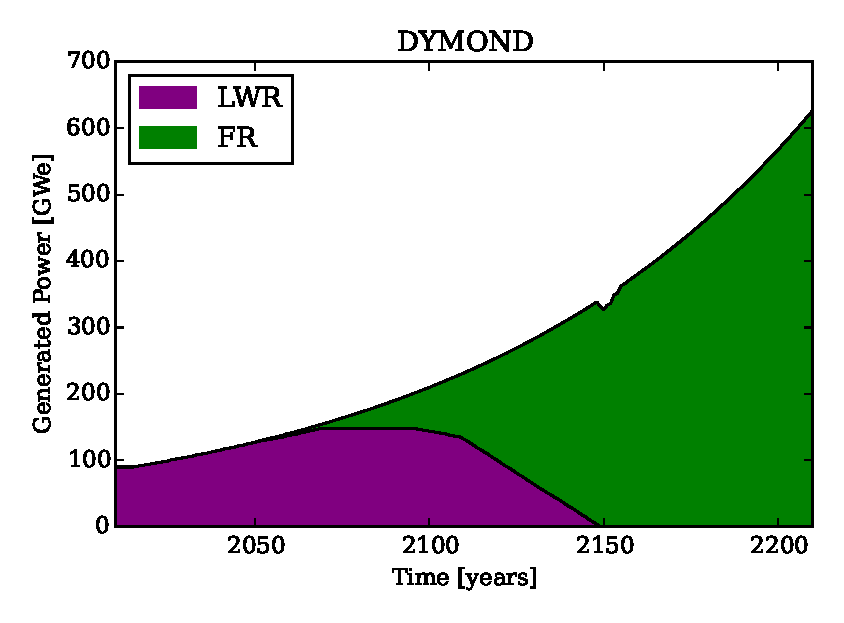
\includegraphics[width=0.45\textwidth]{gwe-dymond.eps}
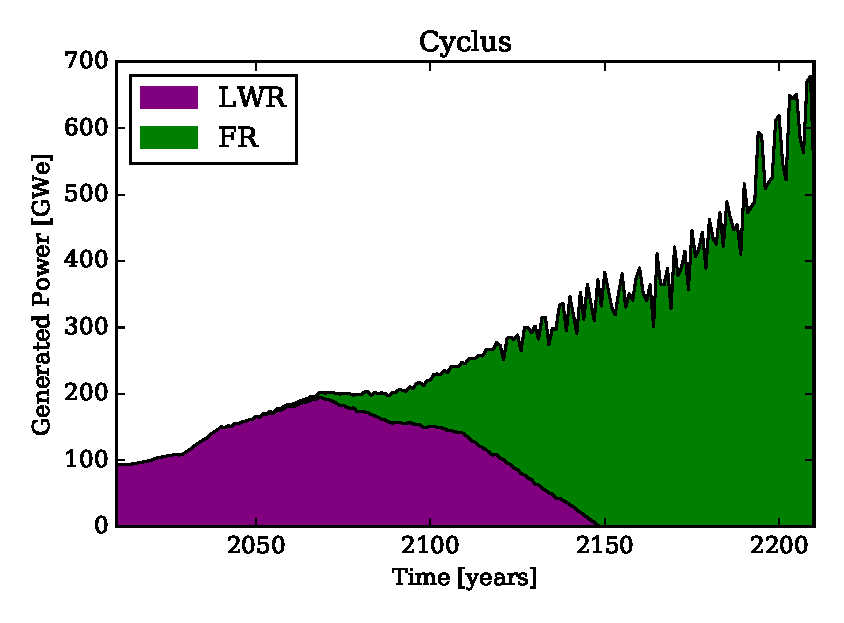
\includegraphics[width=0.45\textwidth]{gwe-cyclus.eps}
\caption{The generated power in [GWe] as a function of time for the DYMOND and 
Cyclus simulators for both LWRs and FRs.}
\label{gwe-simulators}
\end{figure}

\clearpage

\section{Gaussian Process Modeling}
\label{gp}

\section{Dynamic Time Warping}
\label{dtw}

\clearpage
\section{Contribution}
\label{contribution}

In \S\ref{dtw}, the dynamic time warping distance was presented as a 
FOM for measuring the similarity between time series, whether they 
were model-to-simulator comparisons or model-to-model comparisons.
The distances alone, though, have the inverse meaning when trying to 
compute a FOM for contribution to a fuel cycle.  For example, the 
question may be posed as, ``Are LWRs or FRs more important to the fuel 
cycle as a whole?'' While distances can answer this question, smaller 
disantances have higher impact. Preferably, a higher FOM score would yield a 
higher impact. Furthermore, the distances in the previous section have
the same units as the cost matrix and are similarly bounded. A better 
FOM for contribution would be unitless and defined on the range $[0,1]$.

Thus, let $c$ be the \emph{contribution} FOM that satisfies the above 
constraints. To define $c$, first define $D$ as the maximal possible 
distance from the model of the total. Recall that this time series has length $A$.
$D$ is, therefore, the L1 norm of the model of the total time series divided
by twice its length. 
\begin{equation}
\label{D-def}
D(m_*^\Total) = \frac{\left|m_*^\Total\right|_1}{2A}
\end{equation}
This is the equivalent to computing the DTW distance
between $m_*^\Total$ and the curve where the metric is zero for all time 
(i.e. the t-axis itself).  This relies on the notion that 
metric is necessarily non-negative everywhere.  If the metric is allowed to 
be negative, another baseline curve could be chosen. $D$ would then be 
computed as the DTW distance between the total model and this baseline.
However, in most cases the metrics are not allowed to be negative, 
a baseline of zero is suitable, and Equation \ref{D-def} applies.

The contribution figure-of-merit of a given partition to the total is thus 
defined as follows:
\begin{equation}
\label{cont}
c^i = 1 - \frac{d(m_*^\Total, m_*^i)}{D(m_*^\Total)}
\end{equation}
$D$ is seen to normalize the model-to-model distance while subtracting this
ratio from unity makes higher contribution values more important.  
Using the sample data, $c^\LWR = 0.298$ and $c^\FR = 0.859$. This again shows
that the FRs are more important to the total power of the whole cycle.
Here though, higher contribution scores yield higher importance and the values
are always between zero and one.

Note that even though $c$ is a fraction, it is not normalized across 
partitions. Namely, the sum of all contributions for all $I$ partitions
is on the following range, which is not $[0, 1]$:
\begin{equation}
\label{sum-c-range}
0 \le \sum_i^I c^i \le I
\end{equation}
It is easy to imagine an alternative FOM that divides $c^i$ by $I$. However, 
this was not done here because the choice of $I$ (the number of partitions)
can be made arbitrarily large.  In the sample calculations $I=2$ for LWRs and
FRs.  However, $I$ could have been set to 3 by including small modular reactor
(SMRs) which have not yet been built and produce no power.  $I$ could then be 
increased to 4 or higher by including more non-existent reactor types.

Dividing the contribution by $I$ is not sufficient to 
normalize the sum of the $c^i$, in general, because the 
contribution is inherently a cumulative measure. If a component ever had a 
non-zero value, it will always be seen to have contributed something. 
Because of this constraint on the total, $\sum c^i$ can never
reach $I$ unless there is only a single component or the 
total is zero valued everywhere (which implies that the constituents are also 
zero). Thus, dividing $c^i$ by $I$ with the aim of normalizing the 
sum of the $c^i$ is incorrect for any situation of interest to a fuel 
cycle benchmark.

If a truly normalized version of contribution is desired, it must 
use the sum of the actual contributions. Define the normalized contribution 
as $|c^i|$, 
\begin{equation}
\label{norm-ci}
\left|c^i\right| = \frac{c^i}{\sum_j^I c^j}
\end{equation}
The disadvantage with the normalized contribution is that all of the 
individual component $c^i$ must be known prior to the normalization. 
Furthermore, since the sum is typically greater than 1, the difference 
between components is often smaller in the normalized form than in the
more pronounced unnormalized contribution.
The only advantages that $|c^i|$ confers over $c^i$ are that it is defined on 
the range $[0,1]$ and that $\sum |c^i| = 1$. Otherwise, both versions of the FOM
have the same properties with respect to having a zero baseline, the 
intreptation that higher values are higher impact to the total, and that they 
are non-judgmentally derived from models rather than simultors.

\begin{figure}[htb]
\centering
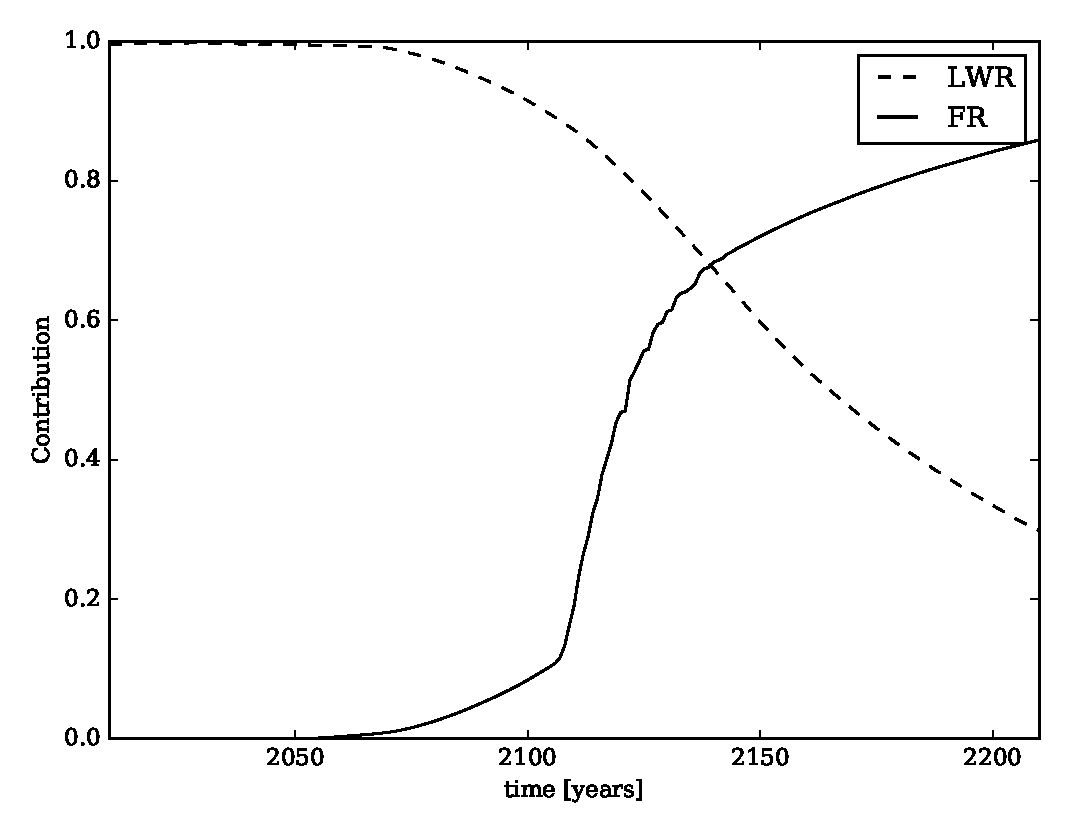
\includegraphics[width=0.9\textwidth]{c-of-t.eps}
\caption{Contribution of LWRs and FRs to total generated power as a 
function of time.}
\label{c-of-t}
\end{figure}

\begin{figure}[htb]
\centering
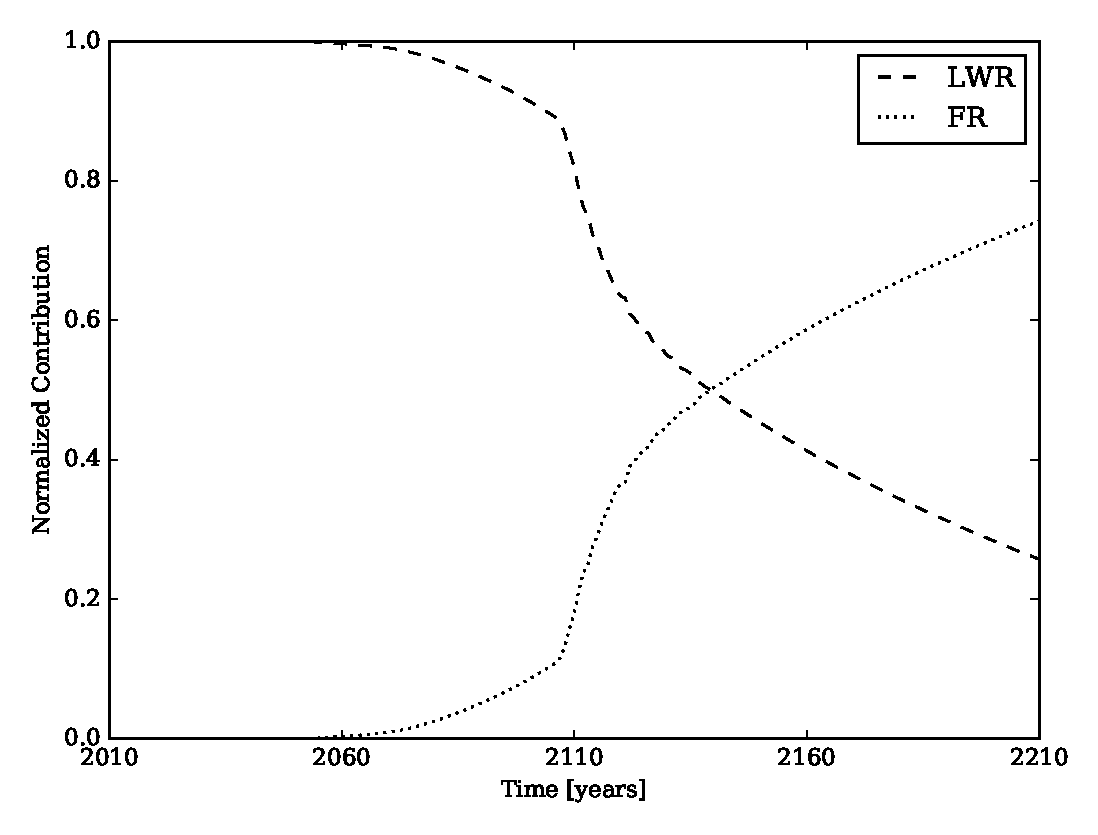
\includegraphics[width=0.9\textwidth]{normc-of-t.eps}
\caption{Normalized contribution of LWRs and FRs to total generated power 
as a function of time.}
\label{normc-of-t}
\end{figure}

Both $c^i$ and $|c^i|$ can be viewed as a function of time.
Doing so in a nuclear fuel cycle benchmark may help identify artifacts in the
calculation that are the result of the time domain chosen for the benchmark itself.
For instance, the FR contribution is expected to overtake the LWR contribution
and this does not occur or occurs very close to the maximum simulation time, 
this implies that the time horizon of the benchmark should be increased.
Figures \ref{c-of-t} \& \ref{normc-of-t} display the contribution and 
normalized contribution respectively for both LWRs and FRs over the full 
time domain. From these figures, the point where FRs become more important 
than LWRs is seen to be approximately year 2140.

\clearpage
\section{Cautionary Tale on Filtering}
\label{filtering}

It is tempting to insert standard filtering techniques from signal processing 
after creating a Gaussian process model but prior to any DTW or contribution 
calculations. A fast Fouier transform (FFT) \citeme based low-pass filter or 
Mel-frequency cepstral coefficients (MFCC) \citeme could be used to reduce error 
in the model itself, 
and thus make the contribution measure more precise. Unfortunately, most 
fuel cycle metrics are not well-formed candidates for such filtering strategies.
Including such filters as part of the analysis can easily lead to wildly unphysical
models.

Consider a simple low-pass filter where a 256 channel real-valued FFT frequency 
transform is taken.  All but lowest 32 channels are discarded prior to the applying 
the inverse transform. High frequency jitter in the original signal is removed, 
allowing for a better signal-to-noise ratio.

\begin{figure}[htb]
\centering
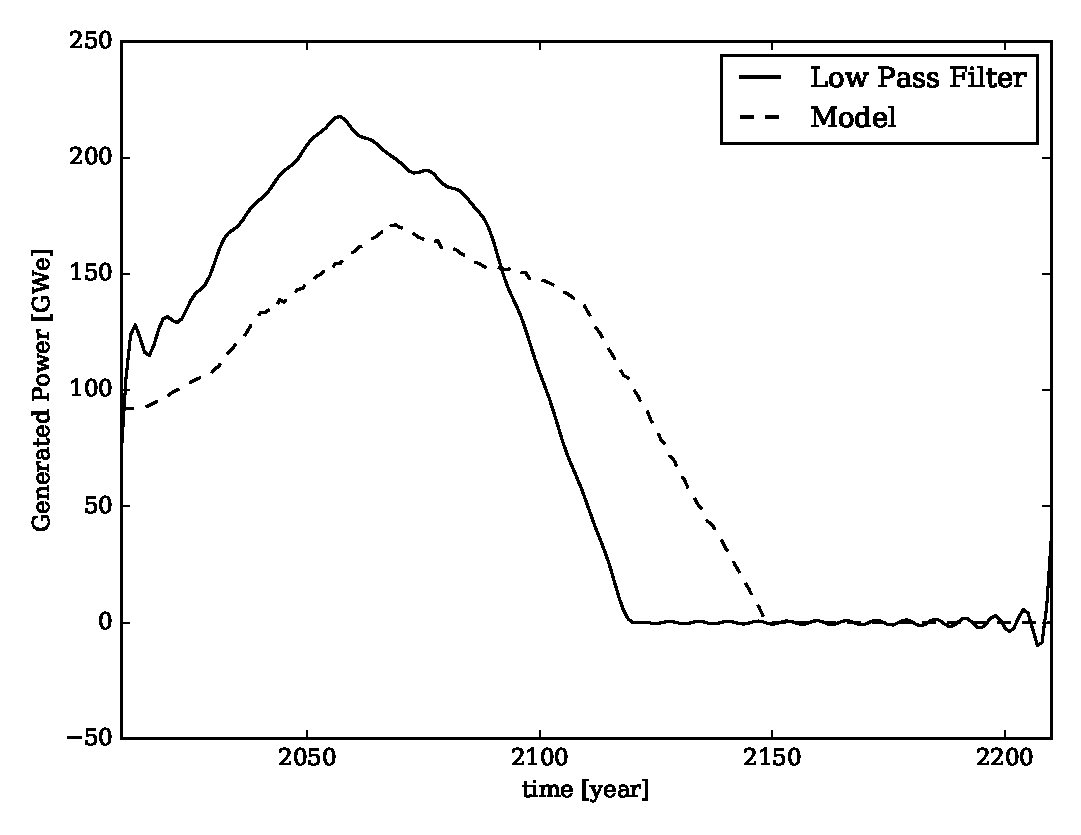
\includegraphics[width=0.9\textwidth]{fft-lwr-model.eps}
\caption{Low-pass FFT filter of LWR Gaussian process model $m_*^\LWR$ alongside
the unfiltered model itself.}
\label{fft-lwr-model}
\end{figure}

Figure \ref{fft-lwr-model} shows the results of applying the low-pass filter 
described above to the Gaussian process model of the generated power from LWRs, 
$m_*^\LWR$.  The filtered curve demonstates at least three major problems.  The
first is that the values of the curve are allowed to be negative, which is 
impossible for this (and many other) fuel cycle metric.  The second is that 
near the time boundaries ($t=2010$ and $t=2210$), the amplitude of the filtered model
is significantly higher than itself. At $t=2210$, the metric should be zero but
instead is 36.5 GWe. Thirdly, the shape of the curve itself is skewed to lower 
times. The time at which the metric goes to zero should be near year 2150 but is 
instead closer to year 2115.  All of these issues would severly distort any 
DTW calculations that follow.

The reason behind these inconsistencies is that the FFT process is fundemenatally 
periodic.  However, using the annual time grid here, most fuel cycle metrics 
are not periodic. Neither is the modeling error for such metrics periodic. 
Thus, while well-intentioned, a low-pass filter is not generally applicable.

Alternatively, MFCCs provide a mechanism for converting a time series into a 
set of power spectrum coefficient curves. Since the dynamic time warping procedure
uses an L1 norm to form the cost matrix, the MFCCs of two signals can be directly 
compared. Each coefficient should roughly correspond in shape and amplitude to some
feature in the original signal.  Noisy, high frequency coeffients tend to be 
very similar and so their contribution to a DTW is less cooresponding less than 
lower coefficients. Coupling MFCC to DTW is an extremely common method employeed in 
speech recognition systems.  

\begin{figure}[htb]
\centering
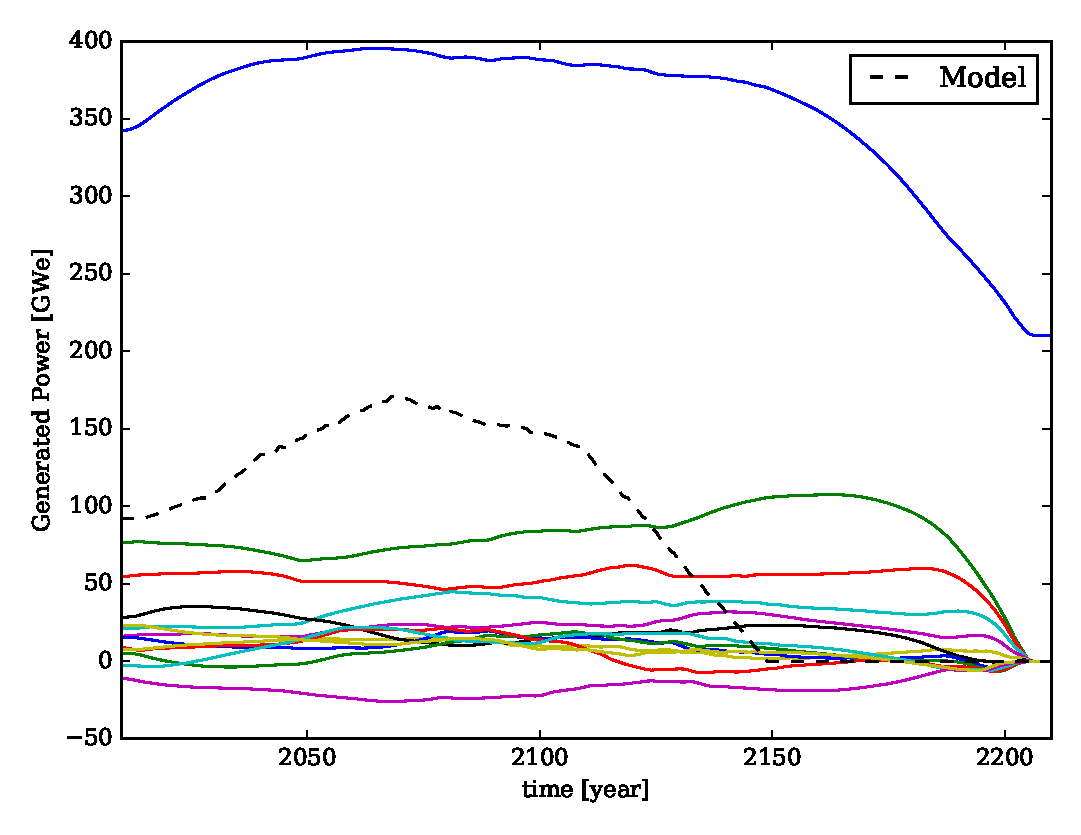
\includegraphics[width=0.9\textwidth]{mfcc-lwr-model.eps}
\caption{Representative Mel-frequency cepstral coefficients (solid lines) of an 
LWR Gaussian process model $m_*^\LWR$ alongside the model itself (dashed line).}
\label{mfcc-lwr-model}
\end{figure}

Figure \ref{mfcc-lwr-model} displays the MFCC curves for the LWR Gaussian 
process model with the model itself. None of these curves, not even the major 
coefficient resembles the actual model.  Rather, the cosine basis for MFCCs
are clearly visible.  As with the low-pass filter, the MFCCs also have 
uncharacteristic negative components.  Moreover, 
the metric data is not sampled frequently enough to have meaningful
time windows. For fuel cycle metrics here, there is one data point per year for 
where the signal itself may change in a meaningful way each year. By comparsion, 
in speech recognition, audio is sampled at least at 22050 hz for charactersitic 
signals on the order of 1 second.  The data volume for fuel cycle benchmark metrics
is simply too low for MFCC transformations to be applicable. 

Still, suppose the contibution measure is computed for the MFCCs of LWR, FR, and 
total generated power models.  In this case the LWR contribution is found to be 
0.572 while the FR contribution is 0.899. Using the models directly as was done 
in \S\ref{contribution}, the contribution values were 0.298 and 0.859 respectively.
This implies that using the MFCCs had the opposite effect as desired.  The MFFCs
added error to the system and mad the LWR and FR contributions seem more alike than 
they truely are.

Therefore filtering the models prior to dynamic time warping is a dubious practice
in the general case. In all likelihood, the metric does not meet the underlying 
assumptions of the filter. The metric may not be periodic or may not be sampled 
frequenctly enough. Sometimes it may be possible to construct as metric that does
meet these qualifcations, such as if the generated power is sampled monthly and 
seasonal demand behaviour is noticable. In such a case, it is instead recomended
to pick a different kernel for the Gaussian process model, such that these 
periodic behaviours are captured.  The regession itself then takes on the role of 
minimizing model uncertainty. Further filtering to this end becomes redundant and
dangerous.  Additionally, it is unlikely that 
the majority of the simulators would be able to calculate such a high-fidelity metric.
That alone should disqulify such a metric from any benchmarking study or
inter-code comparsion.

\section{Conclusions \& Future Work}
\label{conclusion}

This paper demonstrates a robust method for generating figures-of-merit
for nuclear fuel cycle benchmarking activities by coupling Gaussian process
regression to dynamic time warping. This method takes advantage of modeling
uncertainties in fuel cycle metrics if they are known. It is also capable 
of handling the situation where different simulators output metric data on
vastly different time grids. The distance computed by the dynamic time 
warping can itself serve as the figure-of-merit. Additionally, the 
distance can also be used to derive contribution and normalized contribution
figures-of-merit. These measures are valuable for non-judgementally 
determining the impact of different constiuent measures to a total 
metric, e.g. LWR versus FR power generation. The contribution metrics also 
scale such that higher values imply higher impact. This is sometimes
more intuitve as compared to a DTW distance, where lower values imply
more similar curves.

Any regression method could have been used to form a model. Similarly, any
mechanism for comparing two time series could have been used as a measure
of distance.  However, Gaussian processes and DTW were chosen because of 
the nature of a benchmarks and inter-code comparisons that lack experimental
validation. It is not possible to build out a given fuel cycle scenario
and see how it performs 200 years in the future. Furthermore, using 
historical data for validation provides too few cases for comparison and 
each simulator could simply be tuned to precisely match historical events.
Thus, each simulator in a benchmark could be valid or they all could be 
invalid. It is therefore necessary for the FOM to not skew for or against 
any particular simulator. Gaussian process models as used here do not 
judge the simulators differently. The DTW then takes into account the 
cumulative effect of the whole time domain and does not preferentially 
select certain times.

The sample benchmark presented here was very simple and was used for motivation 
purposes only. It consisted of just
two simulators (DYMOND and Cyclus) and one metric (generated power) with
two components (LWR and FR).  However, both Gaussian processes and DTW
are inherently multivariate. More complex forms of analysis could therefore
be performed. For example, the Gaussian process could jointly model the 
effect from many inputs onto the metric. Perhaps the benchmark is formulated
to look at the generated power as a function of time and the power demand curve.
In this case, a two dimensional GP model would be used. Alternatively, 
suppose that a matrix time series of the all individual nuclide mass flows 
are available. DTW is still able compute the distance between two 
such matrices. This would yield a measure of how the mass flows themselves
differ - taking into account each nuclide component - without rely on a collapsed
one dimensional total mass flow curve.  Such cases will be considered in
future work as real inter-code comparison data becomes available.

Furthermore, this work focused on the particular use case of benchmarking.
However, the FOM calculations presented here could also be used to evaluate 
different fuel cycle scenarios. DTW distances could be computed between
a business-as-usual once through scenario and an LWR-to-FR transition
scenario, or any other proposed scenario. This provides a measure for 
comparing the relative cost (in units of the metric, not necessarily 
economic) for selecting one cycle over another. The work here, thus, 
should be seen as a stepping stone to further fuel cycle scenario evaluation
work.

Lastly, dynamic time warping could itself serve a purpose as the objective 
function in a fuel cycle optimization.  For example, suppose a power demand curve 
such as 1\% power growth is known. The DTW distance from the total generated
power to this curve could be minimized as a function of the reactor 
deployment schedule. Such a distance could potentially yield a more 
precise or faster optimization process than simply taking the sum of 
the differences between two time series. Such an optimization would also allow
for matching on multiple time series features simultaneously while retaining
a real-valued objective function.


\section*{Acknowledgements}
\label{acknow}
The author would like to express deep gratitude to Dr. Bo Feng of
Argonne National Lab for providing the DYMOND data used throughout this 
paper.


%%%%%%%%%%%%%%%%%%%%%%%%%%%%%%%%%%%%%%%%%%%%%%%%%%%%%%%%%%%%%%%%%%%%%%%%%%%%%%%%
\bibliographystyle{ans}
\bibliography{refs}
\end{document}
